%%%%%%%%%%%%%%%%%%%%%%%%%%%%%%%%%%%%%%%%%%%%%%%%%%%%%%%%%%%%%%%%%%%%%%%%%%%%%%%%
%2345678901234567890123456789012345678901234567890123456789012345678901234567890
%        1         2         3         4         5         6         7         8

%\documentclass[final,letterpaper, 10 pt, conference]{ieeeconf}  % Comment this line out if you need a4paper

%\documentclass[10pt, conference, compsocconf]{IEEEtran}
%\documentclass[a4paper, 10pt, conference]{ieeeconf}      % Use this line for a4 paper
\documentclass[a4paper, 10pt, conference, compsocconf]{ieeeconf}

\IEEEoverridecommandlockouts                              % This command is only needed if
                                                          % you want to use the \thanks command

\newcommand{\eu}{\textrm{e}}
\newcommand{\figref}[1]{Fig.~\ref{fig:#1}}
\overrideIEEEmargins
\usepackage[obeyFinal]{todonotes}
\RequirePackage{graphicx}
\usepackage{subfigure}
\usepackage{bm}
%\usepackage{subequation}
\graphicspath{ {figures/} }
\usepackage{url}
%\usepackage[tight,footnotesize]{subfigure}
\usepackage{fainekos-macros}
\newcommand{\hatodo}[1]{\todo{HA: #1}}
\newcommand{\hatodoin}[1]{\todo[inline]{HA: #1}}
\newcommand{\sAccu}{\epsilon}
\newcommand{\sDelay}{\delta}
\newcommand{\de}{(\sDelay,\sAccu)}
\newcommand{\dek}[1]{(\sDelay_{#1},\sAccu_{#1})}
\newcommand{\hWc}{\widehat{\Wc}}
\newcommand{\sDelayV}{\underline{\sDelay}}
\newcommand{\sAccuV}{\underline{\sAccu}}
\newcommand{\ESet}{\mathcal{E}}
%\newcommand{\bm}{\hat{B}}
\newcommand{\MPCProb}[1]{\mathbb{P_{#1}}}
\newcommand{\RAMPCProb}[2]{\mathbb{P}_{#1}(\hat{\stPt}_{#2},\sDelay_{#2},\sAccu_{#2},\inpPt_{#2 -1})}

% Set macros
%  outer-approximation
\newcommand{\oa}[1]{\mathbf{#1}}
% inner-approximation
\newcommand{\ua}[1]{\underline{#1}}
% make something nominal
\newcommand{\nom}[1]{\bar{#1}}
% in case we use Z somewhere without subscripts
\global\long\def\Zs{Z}
% Zj,k
\newcommand{\Zset}[2]{\Zs_{#1|#2}}
% set for nominal z
\newcommand{\nomZset}[2]{\nom{\Zset{#1}{#2}}}
% element nominal z
\newcommand{\nomz}[2]{\nom{z}_{#1|#2}}
% e tilde 
\newcommand{\te}{\tilde{e}}
% W hat set
\newcommand{\What}{\widehat{W}}
% X set
\newcommand{\Xset}[2]{X_{#1,#2}}
\newcommand{\such}{\;|\;}

\global\long\def\Cc{\mathcal{C}}
\global\long\def\Nom#1{\overline{#1}}
\newcommand{\bla}[1]{\overbar{#1}}
\newcommand{\bli}[1]{\overline{BLI #1}}
\newboolean{TECH_REPORT}
\setboolean{TECH_REPORT}{FALSE}
\newcommand{\Given}{|}


\newtheorem{theorem}{Theorem}
\newtheorem{corollary}{Corollary}[theorem]
\newtheorem{lemma}[theorem]{Lemma}

\usepackage{array}
\usepackage{url}

\newcommand\Mark[1]{\textsuperscript#1}

% See the \addtolength command later in the file to balance the column lengths
% on the last page of the document

% The following packages can be found on http:\\www.ctan.org
%\usepackage{graphics} % for pdf, bitmapped graphics files
%\usepackage{epsfig} % for postscript graphics files
%\usepackage{mathptmx} % assumes new font selection scheme installed
%\usepackage{times} % assumes new font selection scheme installed
\usepackage{amsmath} % assumes amsmath package installed
\usepackage{amssymb}  % assumes amsmath package installed
%\begin{document}
\title{\LARGE \bf
Co-Design of Anytime Computation and Robust Control
}
%



\title{\LARGE \bf
Robust Model Predictive Control for Non-Linear Systems Feedback Linearization 
}
%
\author{Yash Vardhan Pant, Houssam Abbas, Joseph Devietti, Rahul Mangharam% <-this % stops a space
\thanks{*This work was supported by STARnet a Semiconductor Research
Corporation program sponsored by MARCO and DARPA, NSF MRI-0923518 and the US Department of Transportation University Transportation Center Program}% <-this % stops a space
\thanks{The Departments of Electrical and Systems Engineering and Computer and Information Sciences, University of Pennsylvania, Philadelphia, U.S.A.
        {\small
        \{yashpant,habbas,rahulm\}@seas.upenn.edu, devietti@cis.upenn.edu}}%
}





\begin{document}

\maketitle
\thispagestyle{empty}
\pagestyle{empty}

\section{Problem Formulation} \label{sec:formulation}

The control problem is as follows:

\begin{subequations}
\begin{align}
\text{Minimize } &l(x,u) \\
&\text{s.t.} \nonumber \\
\dot{x}&=f(x)+G(x)u \label{eq:NL_Plant} \\
x&\in X\\
u&\in U
\end{align}
\end{subequations}

Here, $x \in \mathbb{R}^{\dimX}$ and $u \in \mathbb{R}^{\dimU}$. A discrete-time, periodic, state-estimator provides access to a state estimate with estimation error

\begin{subequations}
\label{eq:NL_estimate}
\begin{align}
\hat{x}(t)&=x(t)+e(t) \\ 
\text{where, } e(t) &\in E
\end{align}
\end{subequations}

For sake of simplicity, for the rest of this paper, we assume $X$, $U$ and $E$ are hyper-rectangular, i.e. each dimension of $x$, $u$, $e$ has a fixed upper and lower limit, although the approach we use applies when these 3 sets are convex (bounded) polytopes of arbitrary form.

Given a subset $\Xc$ of a dynamical system's state space, and a horizon $T \geq 0$, the \emph{reachable set of the system from $\Xc$ in time $T$} is the set of states that the system visits, at time $T$ if it starts somewhere in $\Xc$.
Formally, $\RT{\Xc} \defeq \{y \in X \such \exists x_0 \in \Xc: x \text{ is a trajectory of the system, }x(0)=x_0, x(T)=y\}$.

\textbf{Notation}.
Given two subsets $A,B$ of $\Re^n$, define their \textit{Minkowski sum} to be $A\oplus B \defeq \{a+b \such a\in A, b\in B\}$.
Define their Pontryagin difference to be $A\ominus B = \{c \in \Re^n \such c+b \in A\; \forall b \in B\}$
\section{Relating the constraints of successive MPC problems}
\label{sec:set inclusions}

\newcommand{\RT}[1]{RT_{=T}(#1,U)}

%Let $\oa{X_{k+1+j|k+1}}$ be the $j+1$-step reach set computed at time $k+1$ as described in ???.
%Recall that $\oa{X_{k+1+j|k+1}}$ is an outer-approximation of the true reach $X_{k+1+j|k+1}$, which is the set that $x_{k+1+j}$ belongs to if it starts at $x_{k|k}$.

 \subsection{Over-approximating the reach set of the nonlinear system}
\label{sec:x reach}

At time $k$, we need to compute the forward reach set, starting from $x_k$, for the next $N$ steps, for two purposes:
first, this is needed for defining the constraints on the input $v$ to the linearized dynamics.
Secondly, this is needed to compute a containing set for the estimation error in $z$-space.

In all but the simplest systems, forward reachable sets can not be computed exactly.
Moreover, the true state $x_k$ is not known.
Therefore we show how to compute an outer-approximation $\oaXset{k+j}{k},  j=0,\ldots, N$.
To do so we use a reachability tool for nonlinear systems, RTreach??. 
Rtreach computes an outer-approximation of the reachable set of a system starting from some set $\Xc \subset X$, subjet to inputs from a set $U$, for a duration $T \geq 0$. 
Denote this approximation by $\RT{\Xc}$.

At time $k$, the state estimate $\hx_{k}$ is known.
Therefore $x_k = \hx_{k} - e_k \in \hx_{k} \oplus (-E) \defeq \Xset{k}{k}$.
Propagating $\Xset{k}{k}$ forward one step through the continuous-time nonlinear dynamics yields $\Xset{k+1}{k}$, which is outer-approximated by $\RT{\Xset{k}{k}}$.
The estimate that the system will receive at time $k+1$ is therefore bound to be in the set $\RT{\Xset{k}{k}}  \oplus E$.
Since $0 \in E$, we maintain $\Xset{k+1}{k} \subset \RT{\Xset{k}{k}}  \oplus E$.
We define the over-approximate reach set at $k+1$, computed at time $k$, to be 
\begin{equation*}
\label{eq:def Xk}
\oaXset{k+1}{k} \defeq  \RT{\Xset{k}{k}}  \oplus E \oplus  (-E)
\end{equation*}
(The reason for adding the extra $-E$ term will be apparent in the proof to Thm.??).

More generally, for $1 \leq j \leq N$, we define the $j$-step reach set computed at time $k$ to be
\begin{eqnarray}
\label{eq:def Xkj}
\oaXset{k}{k} &\defeq&   \hx_{k} \oplus (-E) 
\nonumber
\\
\oaXset{k+j}{k} & \defeq& \RT{\oaXset{k+j-1}{k}} \oplus E \oplus (-E) 
\end{eqnarray}

The following holds by construction:
\begin{lemma}
	\label{lemma:xreach}
	For any time $k$ and step $j \geq 1$, the $j$-step reach set of the non-linear dynamics starting from $x_k$ is outer-approximated by $\oaXset{k+j}{k}$:
	$\Xset{k+j}{k} \subset \oaXset{k+j}{k}$.
\end{lemma}

This construction of the outer-approximation permits us to prove recursive feasibility of the MPC controller,  because it causes the constraints of the MPC problem setup at time $k+1$ to be consistent with (stronger than) the constraints of the MPC problem setup at time $k$.
This will be explicitly stated and proved in the proof of Thm. ??

\subsection{Approximating the input sets}
\label{sec:approx input sets}
Given $x \in X$, define the set $V(x) \defeq \{v \in \Re^{\dimV} \such u(x) = R^{-1}(x)[b(x)+v] \in U\}$.
We assume that there exist functions $\ua{v}_i, \oa{v}_i: X \rightarrow \Re$ s.t. for any $x$, $V(x) = \{[v_1,\ldots,v_{\dimV}]^T \such \ua{v}_i(x) \leq v_i \leq \oa{v_i}(x) \}$.
Because in general $V(x)$ is not a rectangle, we work with inner and outer rectangular approximations of $V(x)$.
Specifically, let $\Xc$ be a subset of $X$.
Define the inner and outer bounding rectangles, respectively
\[\ua{V}(\Xc) \defeq \{v=[v_1,\ldots,v_{\dimV}]^T \such \max_{x\in \Xc} \ua{v}_i(x)  \leq v_i \leq \min_{x \in \Xc} \oa{v}_i(x) \} \]
\[\oa{V}(\Xc) \defeq \{v=[v_1,\ldots,v_{\dimV}]^T \such \min_{x\in \Xc} \ua{v}_i(x)  \leq v_i \leq \max_{x \in \Xc} \oa{v}_i(x) \} \]

By construction, we have for any subset $\Xc \subset X$
\begin{equation}
\label{eq:Vbounds}
\ua{V}(\Xc) \leq \cup_{x \in \Xc} V(x) \subset \oa{V}(\Xc)
\end{equation}
If two subsets of $X$ satisfy $\Xc_1 \subset \Xc_2$, then it holds that 
\begin{eqnarray}
\label{eq:V inclusions}
\ua{V}(\Xc_2) \subset \ua{V}(\Xc_1)
\nonumber
\\
\oa{V}(\Xc_1) \subset \oa{V}(\Xc_2)
\end{eqnarray}


\subsection{Approximating the  disturbances}
\label{sec:approx dist}
We will also need to define containing sets for the state estimation error in $z$ space:
recall that for any $k,j$, 
$\hat{z}_{k+j} = T(\hat{x}_{k+j}) = T(x_{k+j} + e_{k+j}) \approxeq T(x_{k+j}) + M(x_{k+j})e_{k+j} = z_{k+j} + M(x_{k+j})e_{k+j} = z_{k+j} + \te_{{k+j}}$.
Therefore the state estimation error $\te_{k+j}$ lives in 
$\cup_{x\in X_{k+j|k}, e \in E}M(x)e = \cup_{x \in X_{k+j|k}}M(x)E$, 
where $X_{k+j|k}$ is the $j$-step reach set of the nonlinear dynamics computed starting at time $k$.
%
We over-approximate this set by a rectangle as follows: 
if $\te_{k+j}(i)$ is the $i^{th}$ component of vector $\te_{k+j}$, then 
\[\min_{x \in X_{k+j|k}, e \in E}M_i(x)e \leq \te_{k+j}(i) \leq \max_{x \in X_{k+j|k}, e \in E} M_i(x)e\]
where $M_i(x)$ is the $i^{th}$ row of matrix $M(x)$.
Note we can use $\max$ and $\min$ because the sets $X_{k+j|k}$ and $E$ are closed and bounded so the extrema of the continuous function $M_i(x)e$ are achieved on this set.

Since the set $X_{k+j|k}$ is unknown (we only have access to a state estimate, and the exact reachability computation in general is impossible to perform), we over-approximate it by a reachability tool like ??Rtreach, to obtain $\oa{X}_{k+j|k}$.
Then it holds that 
\[\min_{x \in \oa{X}_{k+j|k} e \in E}M_i(x)e \leq \te_{k+j}(i) \leq \max_{x \in \oa{X}_{k+j|k}, e \in E} M_i(x)e\]

In the examples we use one last over-approximation to simplify the optimizations needed to calculate the component-wise bounds, specifically, we use 
\begin{eqnarray}
\label{eq:Etilde}
\sum_{\ell=1}^{n} \min_{x \in \oa{X}_{k+j|k}, e \in E} M_{i\ell}(x)e(\ell)  \leq \te_{k+j}(i) 
\nonumber 
\\
\leq \sum_{\ell=1}^{n} \max_{x \in \oa{X}_{k+j|k}, e \in E} M_{i\ell}(x)e(\ell)
\end{eqnarray}
where $M_{ij}$ is the $(i,j)^{th}$ element of matrix $M$.
Therefore we define the rectangular error set $\tE_{k+j|k}$ to be the set of vectors $e = [e_1,\ldots, e_{\dimZ}]^T$ satisfying \eqref{eq:Etilde}.

While the sets $\tE_{k}$ over-approximate the mapped estimation error, we also need to calculate containing sets for the process noise $\hat{w}$.
Recall that for all $k,j$, 
$\hz_{k+j+1} = z_{k+j+1} + \te_{k+j+1} = Az_{k+j}+Bv_k+w_{k+j} + \te_{k+j+1} =  A(\hz_{k+j} - \te_{k+j}) + Bv_k + w_{k+j} + \te_{k+j+1} = A\hz_{k+j} + Bv_k + w_{k+j} + \te_{k+j+1} - A \te_{k+j} = A\hz_{k+j} + Bv_k + \hw_{k+j+1}$.

Therefore 
\begin{equation}
\label{eq:What}
\hw_{k+j+1} \in \What_{k+j+1|k} \defeq W \oplus \tE_{k+j+1|k} \oplus(-A\tE_{k+j|k})
\end{equation}

\subsection{Constraints of successive MPC problems}
\label{sec:inclusions statement}
We are now ready to state and prove a key lemma regarding the evolution of the state, error and input sets within one MPC optimization problem, and between MPC optimization problems. 
This lemma will be key to proving recursive feasibility of the MPC controller, since it allows us to show that the constraint sets of one problem, at time $k$, are appropriate supersets of the constraint sets of the next problem, at time $k+1$. 

\begin{lemma}
	\label{lem:set inclusions}
	Let $\oa{X}_{k+j|k}$ be the $j$-step outer-approximate reach set computed at time $k$ by a reachability tool as described in Sec. \ref{sec:x reach}.
	
	Let $\What_{k+j|k}$ be the set defined in \eqref{eq:What}.
	
	Let $\tE_{k+j|k}$ be the error set computed using \eqref{eq:Etilde} by substituting $E \leftarrow \tE_{k|k}$.
	
	Let $\ua{V}_{k+j|k} = \ua{V}(\oa{X}_{k+j|k})$ and $\oa{V}_{k+j|k} = \oa{V}(\oa{X}_{k+j|k})$ 

Then the following hold for all $k \geq 0, ,j \geq 1$:
\begin{enumerate}
	\item $\oa{X}_{k+1+j|k+1} \subseteq \oa{X}_{k+j+1|k}$
	\label{set:X}
	\item $\tE_{k+1+j|k+1} \subseteq \tE_{k+j+1|k}$
	\label{set:tE}
	\item $\What_{k+1+j|k+1} \subseteq \What_{k+j+1|k}$
	\label{set:What}
	\item $\oa{V}_{k+1+j|k+1} \subseteq \oa{V}_{k+j+1|k}$
	\label{set:oaV}
	\item $\ua{V}_{k+1+j|k+1} \supseteq \ua{V}_{k+j+1|k}$ (note the change in inclusion direction)
	\label{set:uaV}		
\end{enumerate} 
%\begin{enumerate}
%		\item $\oa{X}_{k+j+1|k+1} \subseteq \oa{X}_{k+j+1|k}$
%		\item $\tilde{E}_{k+j+1|k+1} \subseteq \tilde{E}_{k+j+1|k}$
%		\item ${W}_{k+j+1|k+1} \subseteq {W}_{k+j+1|k}$
%		\item $\underline{V}_{k+j+1|k+1} \supseteq \underline{V}_{k+j+1|k}$
%		\item $\bar{V}_{k+j+1|k+1} \subseteq \bar{V}_{k+j+1|k}$
%	\end{enumerate}
\end{lemma} 

\begin{proof}
	
\ref{set:X}) 
Fix an arbitrary $k$. We prove this by induction on $j \geq 1$.

\underline{Base case: $j=1$}. By construction, $\hx_{k+1} \in \RT{\Xset{k}{k}} \oplus E$.
Therefore at time $k+1$, when setting up the problem $\mathbb{P}_{k+1}(\hat{z}_{k+1})$, the algorithm will first compute
$\Xset{k+1}{k+1} = \hx_{k+1} \oplus (-E)  \subset \RT{\Xset{k}{k}} \oplus E \oplus (-E) = \oaXset{k+1}{k}$.
Also 
$\oaXset{k+2}{k+1} = \RT{\Xset{k+1}{k+1}} \oplus E \oplus(-E) \subset  \RT{\oaXset{k+1}{k}} \oplus E \oplus(-E) = \oaXset{k+2}{k}$.

\underline{Induction step: $j > 1$}.
By definition, $\oaXset{k+1+j}{k+1} = \RT{\oaXset{k+1+j-1}{k+1}} \oplus E \oplus (-E) \subset  \RT{\oaXset{k+j}{k}} \oplus E \oplus (-E) = \oaXset{k+j+1}{k}$

\ref{set:tE}) 	By \ref{set:X}) 
 we have that 
 $ \min_{x \in \oa{X}_{k+j+1|k}, e \in E} M_{i\ell}(x)e(\ell) \leq \min_{x \in \oa{X}_{k+1+j|k+1}, e \in E} M_{i\ell}(x)e(\ell) \leq $ and 
 $\max_{x \in \oa{X}_{k+j+1|k}, e \in E} M_{i\ell}(x)e(\ell) \leq \max_{x \in \oa{X}_{k+1+j|k+1}, e \in E} M_{i\ell}(x)e(\ell)$
 which yields the desired result.
 
 \ref{set:What}) This is immediate from the definition \eqref{eq:What} and \ref{set:tE}).
 
 \ref{set:oaV}) and \ref{set:uaV}) These are immediate from \eqref{eq:V inclusions}.
 
	\end{proof}

\section{Computing Sets via online reachability}

\subsection{Online reachability and overapproximation}

As seen in Section \textbf{setdefs}, we need $X_{k}$ in order to compute the inner convex bound on the input $v$ at time $k$, $\underline{V}_k$, and also to compute the bounding set for the estimation error $\tilde{e}_k$, $\tilde{E}_k$. For our Robust Model Predictive Controller, we will need these sets for the length of the MPC horizon starting at time $k$, i.e. for time $k=0,\dotsc,N$. For the purpose of getting these sets for future inputs and estimation errors starting at time $k$, we compute an outer-approximation of the reachable sets for the non-linear system,  $\bar{X}_{k+j|k})$ starting at time $k$.

For $j=0$, given the state estimate $\hat{x}_k$,  we have the set ${X}_{k|k}$ where the true state $X_k$ can lie, given as $X_{k|k} = \lbrace \hat{x}_k \rbrace \oplus (-E)$ since we know $\hat{x}_k = x_k + e_k$ and $e_k \in E$. Next, we compute the set of reachable states at time step $k+1$ starting from all states in ${X}_{k|k}$ and all inputs in $u \in U$. From this set, we make an over-approximation by adding (in the sense of Minkowsi Sum), $-E$ and $E$,  i.e. $\bar{X}_{k+1|k} = \text{Reach}_h(X_{k|k},U)\oplus(-E) \oplus(E)$. the reason for this over-approximation will become clearer later in this section. So for the sets in which $x_{k+j}$ can lie, given the state estimate at time $k$, we have $\forall j=0,\dotsc,N$
\begin{subequations}
\label{eq:overreach_NL}
\begin{align}
\bar{X}_{k|k}&=X_{k|k}=\lbrace\hat{x}_k\rbrace \oplus (-E) \\
\bar{X}_{k+j|k}&=Reach_h(\bar{X}_{k+j-1},U) \oplus (-E) \oplus (E) \forall j=1,\dotsc,N
\end{align}
\end{subequations}

We explain the reason behind the approximation via Figure \ref{fig:overreach_NL}. For $j>0$, we add (in the sense of Minkowski sum) $(-2E)$ to the set obtained via reachability in order to ensure that the over-approximated reachable sets computed for the same time instant $k+j$ at the next time step $k+1$ through Eq. \ref{eq:overreach_NL}, $\bar{X}_{k+j|k+1}$ are such that 

\begin{equation}
\label{eq:reach_contain}
\bar{X}_{k+1+j|k+1} \subseteq \bar{X}_{k+1+j|k}
\end{equation}

Note, for time step $k+1$, $Reach_h(\bar{X}_{k|k},U)$ gives us the set where the actual state $x_k$ can lie. Since $\hat{x}_k = x_k+e_k$, $Reach_h(\bar{X}_{k|k},U) \oplus (E)$ gives us the set where the state estimate at time $k+1$, $\hat{x}_{k+1}$ can lie. Finally $Reach_h(\bar{X}_{k|k},U) \oplus (E) \oplus (-E)$ gives us a set in which $\lbrace \hat{x}_{k+1} \rbrace \oplus (-E)$, i.e. $\bar{X}_{k+1|k+1}$. At the next time step $k+2$, we similarly add $\oplus (-E)\oplus (E)$ to the set obtained from reachability on $\hat{X}_{k+1|k+1}$ becase we want the set computed at time $k+1$ via reachability on $\bar{X}_{k+1|k+1}$ to lie inside it and so on for other time steps. This gives us Eq. \ref{eq:reach_contain} $\forall k$ by following the reachability over approximations of Eq. \ref{eq:overreach_NL}.

Given this approach, at time $k$, we have an over-approximation of the set in which $x_{k+j}$ lies for all $j=0,\dotsc,N$. These sets can be computed via online reachability algorithms in real-time, e.g. \textbf{RTReach}.

\subsection{Computing bounding sets for $v$ and $\tilde{e}$ online}

By computing the sets $\bar{X}_{k+j|k}$, we can use compute $\tilde{E}_{k+j}$ and $\underline{V}_{k+j}$ online using the definition of these sets. We have $\forall j=0,\dotsc,N$

\begin{equation}
\tilde{E}_{k+j|k}  = \cup_{x \in \bar{X}_{k+j|k}}M(x)E
\end{equation}

And, 

\begin{equation}
\underline{V}_{k+j|k} = \lbrace v|u\in U, \, \forall x \in \bar{X}_{k+j|k} \rbrace
\end{equation}



\begin{figure*}
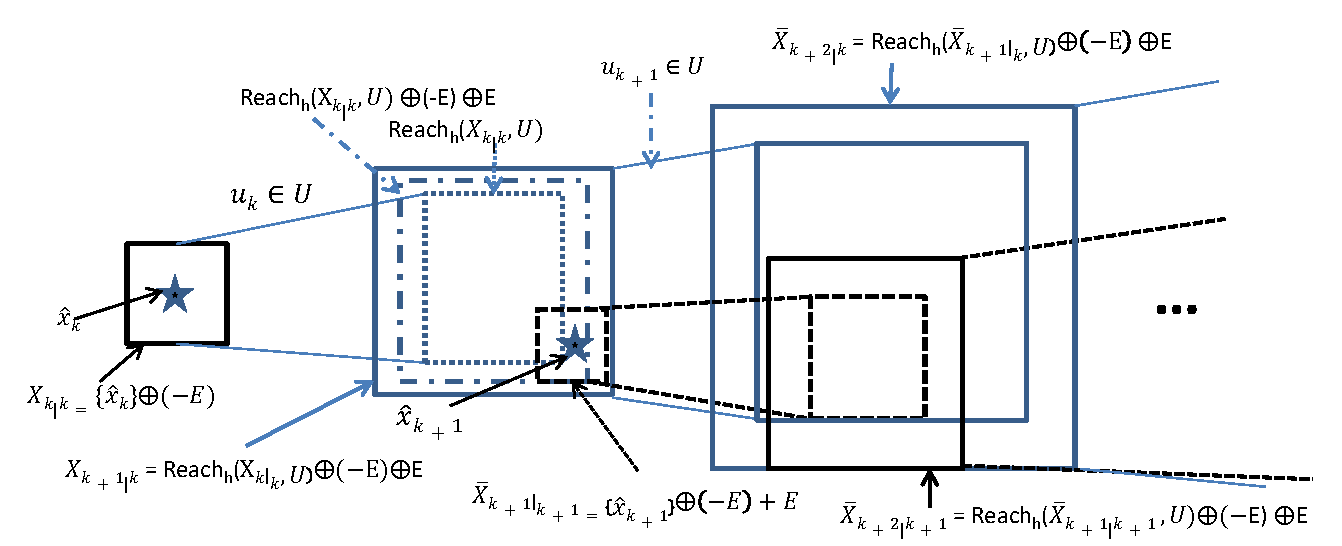
\includegraphics[scale=0.75]{figs/OverReachFigure_NL_scissored.pdf}
\caption{The over-approximated reachable sets for $x_{k+j}$, computed at time steps $k$, and correspondingly ay $k+1$ , used to compute $\tilde{E}_{k+j|k}$, $\underline{V}_{k+j|k}$. }
\label{fig:overreach_NL}
\end{figure*}
\section{Robust MPC for the feedback linearized system}
\label{sec:feedback lin rmpc}

Following \cite{RichardsH05_RMPC}, \cite{PantAMNDM15_Anytime}, we formulate a Robust MPC (RMPC) controller of \eqref{eq:discrete linear problem} via \emph{constraint restriction}.
We outline the idea before providing the technical details.
The key idea is to move the effects of estimation error $\tilde{e}_k$ and  process noise $w_k$ (the `disturbances') to the constraints, and work with the nominal  (i.e., disturbance-free) dynamics: $\nz_{k+1} = A\nz_{k}+Bv_k$, $\nz_{0} = \hat{z}_0$.
Because we would be optimizing over disturbance-free states, we must account for the noise in the constraints. 
Specifically, rather than require the next (nominal) state $\nz_{k+1}$ to be in $Z$, we require it to be in the shrunk set $Z \ominus \What_{k+1|k} \ominus \tE_{k+1|k}$: 
by definition of Pontryagin difference, this implies that whatever the actual value of the noise $\hw_{k+1} \in \What_{k+1|k}$ and of the estimation error $\tilde{e}_{k+1} \in \tE_{k+1|k}$, the actual state $z_{k+1}$ will be in $Z$. 
This is repeated over the entire MPC prediction horizon $j=1,\ldots,N$, with further shrinking at every step.
For further steps ($j>1$), the process noise $\hw_{k+j|k}$ is propagated through the dynamics, so the shrinking term $\What$ is shaped by a stabilizing feedback controller $\nz \mapsto K\nz$.
At the final step ($j=N+1$), a terminal constraint is derived using the worst case estimation error set $\tE_{max}$ and a global inner approximation for the input constraints, $V_{inner-global}$. 

Through this successive constraint tightening we ensure robust safety and feasibility of the feedback linearized system (and hence of the non-linear system). 
Since we use just the nominal dynamics, and show that the tightened constraints are linear in the state and inputs, we still solve a Quadratic Program (QP) for the RMPC optimization.
The difficulty of applying RMPC in our setting is that the amounts by which the various sets are shrunk vary with time because of the time-varying state estimation error, are state-dependent, and involve set computations with the non-convexity preserving mapping $T$.
One of our contributions in this paper is to establish recursive feasibility of RMPC with time-varying constraint sets.

The RMPC optimization $\Pk{k}$ for solving \eqref{eq:discrete linear problem} is:
\begin{subequations} 
\label{eq:nom mpc}
\begin{align}
J^{*}(\nz_{k}) &= \min_{\mathbf{\nz},\mathbf{u}} \sum_{j=0}^{N}\lbrace \nz_{k+j|k}^{T}Q \nz_{k+j|k} + {v}_{k+j|k}^{T}R{v}_{k+j|k}\rbrace \nonumber \\ 
                    &\quad  +  \nz_{k+N+1|k}^T Q_f \nz_{k+N+1|k}  \label{eq:cost} \\
\nz_{k|k}       &= \hat{z}_{k} \label{eq:init_cond}\\
\nz_{k+j+1|k} &=A\nz_{k+j|k} + Bv_{k+j|k} , j=0,\ldots,N\label{eq:nom_dyn} \\
\nz_{k+j|k}     & \in \nomZset{k+j}{k} , \; j=0,\ldots,N \label{eq:states_con}\\
v_{k+j|k}        & \in  V_{k+j|k} , \;j=0,\ldots,N-1 \label{eq:input_con} \\
p_{N+1}               &= \lbrack z_{k+N+1|k} , v_{k+N|k} \rbrack^{T}  \in P_f \label{eq:joint_term} 
	\end{align}
\end{subequations}

Here, $\nz$ is the state of the nominal feedback linearized system.
The cost and constraints of the optimization are explained below:
\begin{itemize}
\item Eq. \eqref{eq:cost} shows a cost quadratic in $\nz$ and $v$, where as usual $Q$ is positive semi-definite and $R$ is positive definite. 
In the terminal cost term, $Q_f$ is the solution of the Lyapunov equation $Q_f-(A+BK)^{T}Q_f(A+BK) = Q+K^{T}RK$.
This choice guarantees that the terminal cost equals the infinite horizon cost under a linear feedback control $\nz \mapsto K\nz$ \cite{CannonK15MPC}.

\item Eq. \eqref{eq:init_cond} initializes the nominal state with the current state estimate.

\item Eq. \eqref{eq:nom_dyn} gives the nominal dynamics of the discretized feedback linearized system.

\item Eq. \eqref{eq:states_con} tightens the admissible set of the nominal state by a sequence of shrinking sets.

\item Eq. \eqref{eq:input_con} constrains $v_{k+j|k}$ such that the corresponding $u(x,v)$ is admissible, and the RMPC is recursively feasible.

\item Eq. \eqref{eq:joint_term} constrains the final input and nominal state to be within a terminal set $P_f$.

\end{itemize}

The details of these sets' definitions and computations are given in Sec. \ref{sec:set definitions}.

\subsection{State and Input Constraints for the Robust MPC}

The state and input constraints for the Robust MPC are as defined as follows:

\textit{The state constraints $Z_{j|k}$:}
The tightened state constraints are functions of the error sets $E_{k+j|k}$, and defined $\forall\,j=0,\dotsc,N$
\small{
\begin{subequations} \label{eq:Set_constraints}
\begin{align}
Z_{0|k}(\tilde{E}_{k|k}) &=Z\ominus(-\tilde{E}_{k|k}) \\
Z_{j+1|k}(\tilde{E}_{k+j+1|k},\tilde{E}_{k+j|k}) &= Z_{j|k}(\tilde{E}_{k+j+1|k},\tilde{E}_{k+j|k})\ominus L_{j}W_{k+1|k}
\end{align}
\end{subequations}}

Here, the matrix $L_j$, $\forall j=0,\dotsc,n$   is defined as
\begin{subequations} \label{eq:L_def}
\begin{align}
L_0&=\mathbb{I} \\
L_{j+1} &= (A+BK)L_j
\end{align}
\end{subequations}

\textit{The input constraints $V_{j|k}$:}
The input constraints are given, $\forall j=0,...,N-1$, as:

\begin{subequations}
\begin{align}
V_{0|k} = \underline{V}_{k|k} \\
V_{j+1|k} = \underline{V}_{k+j+1|k} \ominus KL_jW_{k+1|k}
\end{align}
\end{subequations}

\textit{The terminal constraint $Z_f$:}
For the terminal constraint, which is a joint constraint on both the input and the nominal state, let us first define a few terms.
\begin{subequations}
\begin{align}
p_k &=[z_k \, v_{k-1}]' \label{eq:joint_state} \\
\hat{A} &= \begin{bmatrix} A & 0_{nxm} \\ 0_{mxn} & 0_{mxm}   \end{bmatrix} \label{eq:A_hat} \\
\hat{B} &= \begin{bmatrix}  B \\ \mathbb{I}_{mxm} \end{bmatrix} \label{eq:B_hat} \\
\hat{K} &= \begin{bmatrix}  K & 0_{mxm}  \end{bmatrix} \label{eq:K_hat} \\
\hat{L} &= \hat{A}+\hat{B}\hat{K} \label{eq:L_hat} \\
\hat{F} &= \begin{bmatrix} \mathbb{I} \\ 0_{mxn} \end{bmatrix} \\
W_{max} &= W \oplus \tilde{E}_{max} \oplus (-A\tilde{E}_{max}) \label{eq:W_max} 
\end{align}
\end{subequations}

Here, $p_k$ is a state formed by concatenating the state at time $k$ and the input at time $k-1$ (Eq.(\ref{eq:joint_state})). $\hat{A}$, $\hat{B}$, define the dynamics of the new state $p_{k+1} = \hat{A}p_{k} + \hat{B}v_k$. $\hat{L}$ is defined as $L$ is in Eq.(\ref{eq:L_def}). Also, similar to $K$, which is a stabilizing state feedback matrix for the system defined by $A$ and $B$, $\hat{K}$ acts as a stabilizing matrix for the system given by $\hat{A}$ and $\hat{B}$.

With these definitions, $Z_f$ is defined as:
\begin{equation}
Z_f = C\ominus \hat{L}_N\hat{F}{W}_{max}
\end{equation}

Here, $C$ is a robust control invariant set for the worst case disturbances given by $W_{max}$. Note. $C$ is the invariant set inside $\hat{Z}_N(\tilde{E}_{max},\tilde{E}_{max})$, where $\hat{Z}_N(\tilde{E}_{max},\tilde{E}_{max})$ is computed recursively, similar to Eq. \ref{eq:Set_constraints} but with all error sets replaced by $\tilde{E}_{max}$ as follows $\forall j=0,\dotsc,N$


\begin{subequations}
\begin{align}
\hat{Z}_0(\tilde{E}_{max}) &=\hat{Z}\ominus(-\tilde{E}_{max}) \\
\hat{Z}_j(\tilde{E}_{max},\tilde{E}_{max}) &= \hat{Z}_j(\tilde{E}_{max},\tilde{E}_{max})\ominus \hat{L}_{j}W_{max}
\end{align}
\end{subequations}

Where $\hat{Z}=Z\times V_{inner-global}$. The robust control invariant set inside $Z_N(\tilde{E}_{max},\tilde{E}_{max})$, $C$ is such that there exists a feedback control law $v=\hat{K}p$, such that $\forall p\in C$


\begin{subequations}
\begin{align}
\hat{A}z &+ \hat{B}Kp+L_N \hat{F}w \, \in C,\, \forall w \in W_{max} \\
p \in &\hat{Z}_N(\tilde{E}_{max}, \tilde{E}_{max})
\end{align}
\end{subequations}

It is worth noting, that this set is computed offline since it depends on the worst case disturbances $W_{max}$, $E_{max}$ and the global inner convex approximation for the constraints on $v$, $V_{inner-global}$ which can be all be computed offline. With this conservative approximation of the shrinking sets, it is obvious that this is indeed invariant for all disturbance sets, $\forall j$, $E_{k+j|k}$ and $W_{k+j|k}$, which both are contained in $E_{max}$, $W_{max}$ respectively. 


\subsection{The Control Algorithm}
\label{sec:the control algo}
We can now describe the algorithm used for solving \eqref{eq:generic NLMPC} by robust receding horizon control of the feedback linearized nominal dynamics.

\begin{algorithm}
	\caption{RMPC via feedback linearization}
\begin{algorithmic}
	\Require System model, $X$, $U$, $E$, $W$ 
	\State	Offline, compute:
	\State \quad Initial safe sets $X_0$ and $Z$ \Comment{Sec. \ref{sec:transforming x to z}}
	\State \quad $\tE_{max}$, $\What_{max}$ \Comment{Sec. \ref{sec:approx dist} }
	\State \quad $C_p$, $P_f$ \Comment{Sec. \ref{sec:Constraints}}
	\State Online: 
	\If{$P_f = \emptyset$}
	\State Quit
	\Else
	\For{$k=1,2,\ldots$}
	\State Compute $\ua{V}_{k+j|k},\,\tE_{k+j|k},\, \What_{k+j|k}$ \Comment{Sec. \ref{sec:approx input sets}}
	\State Compute $\nomZset{k+j}{k},\,V_{k+j|k}$ \Comment{Sec. \ref{sec:Constraints}}
	\State $(v^*_{k|k}, \ldots, v^*_{k+N|k}) = $ Solution of $\Pk{k}$ 
	\State $v_k = v^{*}_{k|k}$
	\State Apply $u_k = R(\hx_{k}^{-1})[b(\hx_{k})+v_k]$ to plant 
	\EndFor	
	\EndIf		
\end{algorithmic}
\label{alg:RMPC}
\end{algorithm}



\subsection{Robust Feasibility and Stability}
We are now ready to state the main result of this paper: namely, that the RMPC of the feedback linearized system \eqref{eq:nom mpc} is feasible at all time steps if it starts out feasible, and that it stabilizes the nonlinear system, for all possible values of the state estimation error and feedback linearization error.

\begin{theorem}[Robust Feasibility]
\label{th:robust_feas}
If at some time step $k_0 \geq 0$, the RMPC optimization $\Pk{k_0}$ is feasible, then all subsequent optimizations  $\Pk{k} k> k_0$ are also feasible.
Moreover, the nonlinear system \eqref{eq:generic NLMPC} controlled by algorithm \ref{alg:RMPC} and subject to the disturbances ($E$, $W$) satisfies its state and input constraints at all times $k \geq k_0$.
\end{theorem}


\begin{theorem}[Stability]
%	\label{thm:stability}
%Given an equilibrium point $x_e \in X_0 \subset \iT(Z)$ of the nonlinear dynamics \eqref{eq:generic NLMPC}, Algorithm \ref{alg:RMPC} stabilizes the nonlinear system to $x_e$.
%\end{theorem}
	\label{thm:stability}
Given an equilibrium point $x_e \in X_0 \subset \iT(Z)$ of the nonlinear dynamics \eqref{eq:generic NLMPC}, Algorithm \ref{alg:RMPC} stabilizes the nonlinear system to an invariant set around $x_e$.
\end{theorem}

\begin{proof}
Let $T$ be the diffeomorphism mapping $x$ to $z$ from feedback linearization.
By a change of variables $z' = z - T(x_e)$, stabilizing the linear dynamics (with state $z'$) to 0 implies stabilizing the nonlinear dynamics to $x_e$.
Recall that $Q$ and $Q_f$ of  \eqref{eq:nom mpc} are positive definite and that $R$ is positive semi-definite,  so that the optimal cost $J^*(\nz_{k})$ is a positive definite function of $\nz_{k}$, and that the terminal weight in \eqref{eq:nom mpc} is equivalent to the infinite horizon cost (by our choice of $Q_f$). 
Finally Thm.  \ref{th:robust_feas} guarantees that the tail of the input sequence computed at $k$ is admissible at time $k+1$. 
Therefore it is a standard result that the optimal cost $J^{*}({\nz}_{k})$ is non-increasing in $k$ and that $0$ is a stable equilibrium for the closed-loop linear system (e.g., see \cite{CannonK15MPC} ). 
Moreover the nominal feedback-linearized system ($\nz$) converges to 0 from anywhere in $Z$. Therefore, the nominal $\bar{x}_{k}$ converges to $x_e$ from anywhere in $X_0 \subset \iT(Z)$. The true state ($x_k$) then converges to the invariant set around $x_e$.
\end{proof}
\section*{Appendix}
\label{appendix}

In this appendix we give the detailed mathematical derivation of the results of Section \ctrlProbSecRef.
The controller is designed using a Robust Model Predictive
Control (RMPC) approach via constraint restriction \cite{richardsetal05rmp, chiscietal01swp}, 
and augments it by an adaptation to the error-delay curve of the estimator.
In order to ensure robust safety and feasibility, the key idea of
the RMPC approach is to tighten the constraint sets iteratively to account
for possible effect of the disturbances. 
As time progresses, this ``robustness
margin'' is used in the MPC optimization with the nominal dynamics,
i.e., the original dynamics where the disturbances are either removed
or replaced by nominal disturbances.
%An advantage of this approach is that, 
Because only the nominal dynamics are used, the complexity of the optimization is the same as for the nominal problem.

Since the controller only has access to the estimated state $\hat{x}$, we need
to rewrite the plant's dynamics with respect to $\hat{x}$. 
The error
between $ $$x_{k}$ and $\hat{x}_{k}$ is $e_{k}=x_{k}-\hat{x}_{k}$.
At time step $k+1$ we have
\begin{align*}
\hat{x}_{k+1} & =x_{k+1}-e_{k+1}\\
 & =Ax_{k}+B_{1}(\sDelay_k)u_{k-1}+B_{2}(\sDelay[k])u_{k}+w_{k}-e_{k+1}\text{,}
\end{align*}
 then, by writing $x_{k}=\hat{x}_{k}+e_{k}$, we obtain the dynamics
\begin{equation}
\hat{x}_{k+1}=A\hat{x}_{k}+B_{1}(\sDelay[k])u_{k-1}+B_{2}(\sDelay[k])u_{k}+\hat{w}_{k}\label{eq:estimator-dynamics}
\end{equation}
 where $\hat{w}_{k}=w_{k}+Ae_{k}-e_{k+1}$.
The set of possible values of $\hat{w}_{k}$
depends on the estimation accuracy at steps $k$ and $k+1$ and is
denoted by $\hWc(\sAccu[k],\sAccu[k+1])$, i.e.,
$\hWc(\sAccu,\sAccu')\defeq \left\{ w+Ae-e'\sut w\in\Wc,e\in\ESet(\sAccu),e'\in\ESet(\sAccu')\right\}$.
Note that %we assume
$\hWc(\sAccu[k],\sAccu[k+1])$ is independent
of the time step $k$. %
It can be computed as $\hWc(\sAccu,\sAccu')=\Wc\oplus A\ESet(\sAccu)\oplus\left(-\ESet(\sAccu')\right)$
where the symbol $\oplus$ denotes the Minkowski sum of two sets.

The dynamics in \eqref{eq:estimator-dynamics} has a non-standard form
where it depends on both the current and the previous control inputs.
However we can expand the state variable to store the previous control
input as
\[
\hat{z}_{k}=\begin{bmatrix}\hat{x}_{k}\\
u_{k-1}
\end{bmatrix}\in\Re^{n+m}
\]
and rewrite the dynamics as, for all $k\geq0$,
\begin{equation}
\hat{z}_{k+1}=\hat{A}(\sDelay_k)\hat{z}_{k}+\hat{B}(\sDelay_k)u_{k}+\hat{F}\hat{w}_{k}\text{.}\label{eq:estimator-std-dynamics}
\end{equation}
Here, the system matrices are
\begin{equation}
\begin{gathered}
\hat{A}(\sDelay_k)=\begin{bmatrix}A & B_{1}(\sDelay_k)\\
\bm{0}_{m\times n} & \bm{0}_{m\times m}
\end{bmatrix},\\
\hat{B}(\sDelay_k)=\begin{bmatrix}B_{2}(\sDelay_k)\\
\IdentityMatrix_{m}
\end{bmatrix},\quad\hat{F}=\begin{bmatrix}\IdentityMatrix_{n}\\
\bm{0}_{m\times n}
\end{bmatrix}\text{.}
\end{gathered}
\label{eq:lifted-matrices}
\end{equation}

Let the actual expanded state be $z_{k}=\left[x_{k}^{T},u_{k-1}^{T}\right]^{T}$.
Because the expanded state consists of both the plant's state and
the previous control input, the state constraint $x_{k}\in\stSet$
and the control constraint $u_{k}\in\inpSet$ are equivalent to the
joint constraint $z_{k}\in\stSet\times\inpSet$. We can now describe
the RAMPC algorithm for the dynamics in \eqref{eq:estimator-std-dynamics}.

\subsection{Tractable RAMPC Algorithm}

Let $N\geq1$ be the horizon length of the RMPC optimization. 
Because the system
matrices in the state equation~(\ref{eq:estimator-std-dynamics})
depend nonlinearly on the variables $\sDelay_k$, the RMPC optimization
is generally a mixed-integer nonlinear program, which is very hard
to solve. To simplify the RMPC optimization to make it tractable, we fix the estimation mode for the entire RMPC horizon.

Let $\RAMPCProb{\de}{k}$
denote the RMPC optimization problem at step $k\geq0$ where the current
state estimate is $\hat{x}_{k}$, the current estimation mode is $(\sDelay_k,\sAccu_k)\in\Delta$,
the previous control input is $u_{k-1}$, and the estimation mode
for the entire horizon (after step $k$) is fixed at $(\sDelay,\sAccu)\in\Delta$.
Since the system matrices become constant now, if the stage cost $\ell(\cdot)$
is linear or positive semidefinite quadratic, each optimization problem
$\RAMPCProb{\de}{\cdot}$ is tractable and can be solved
efficiently as we will show later. 
The RAMPC algorithm with Anytime Estimation is stated in Alg. \algoref.

\subsection{RMPC Formulation}

We formulate the RMPC optimization $\RAMPCProb{\de}{k}$
with respect to the nominal dynamics, which is the original dynamics
in \eqref{estimator-std-dynamics} but the disturbances are either
removed or replaced by nominal disturbances. 
To ensure robust feasibility
and safety, the state constraint set is tightened after each step
using a candidate stabilizing state feedback control, and a terminal
constraint is derived. 
In this RMPC formulation, we extend the approach
in \cite{richardsetal05rmp, chiscietal01swp}. 
At time step $k$, given
$(\hat{x}_{k},\sDelay_k,\sAccu_k,u_{k-1})$ and for a fixed $(\sDelay,\sAccu)$,
we solve the following optimization 

\begin{subequations}
	\label{eq:RMPC1}
 \begin{equation} J_{\sDelay,\sAccu}^{*} \left(\hat{x}_{k},\sDelay_k,\sAccu_k,u_{k-1}\right) = \min_{\boldsymbol{u},\boldsymbol{x}}\sum_{j=0}^{N}\ell(\Nom x_{k+j\Given k},u_{k+j\Given k})
 \end{equation}
 \begin{equation}
  \text{subject to, }\forall j\in\left\{ 0,\dots,N\right\} \nonumber 
 \end{equation}
 \begin{equation}
  \Nom z_{k+j+1\Given k}=\hat{A}(\sDelay_{k+j\Given k})\Nom z_{k+j\Given k}+\hat{B}(\sDelay_{k+j\Given k})u_{k+j\Given k}\label{eq:RMPC1-dyn}
 \end{equation}
 \begin{equation}
  ( \sDelay_{k+j+1\Given k},\sAccu_{k+j+1\Given k} ) \!=\! (\sDelay,\sAccu ) \nonumber
 \end{equation}
 \begin{equation}
  (\sDelay_{k\Given k},\sAccu_{k\Given k}) \!=\! (\sDelay_k,\sAccu_k)  \label{eq:RMPC1-delay}
 \end{equation}
 \begin{equation}
  \Nom x_{k+j\Given k}=\begin{bmatrix}\IdentityMatrix_{n} \quad \bm{0}_{n\times m}\end{bmatrix}\Nom z_{k+j\Given k}\label{eq:RMPC1-z2x}
 \end{equation}
 \begin{equation}
  \Nom z_{k\Given k}=\left[\hat{x}_{k}^{T},u_{k-1}^{T}\right]^{T} \label{eq:RMPC1-z0}
 \end{equation}
 \begin{equation}
  \Nom z_{k+j\Given k}\in\ZSet_{j}\left(\sAccu_k,\sAccu\right)\label{eq:RMPC1-zset}
 \end{equation}
 \begin{equation}
  \Nom z_{k+N+1\Given k}\in\ZSet_{f}\left(\sAccu_k,\sAccu\right) \label{eq:RMPC1-zfinalset}
  \end{equation}
\end{subequations} 

in which $\Nom z$ and $\Nom x$
are the variables of the nominal dynamics. The constraints of the
optimization are explained below.
\begin{itemize}
\item \eqref{eq:RMPC1-dyn} is the nominal dynamics.
\item \eqref{eq:RMPC1-delay} states that the estimation mode is fixed at $\left(\sDelay,\sAccu\right)$
except for the first time step when it is $\left(\sDelay_k,\sAccu_k\right)$.
\item \eqref{eq:RMPC1-z2x} extracts the nominal state $\Nom x$ of the plant
from the nominal expanded state $\Nom z$.
\item \eqref{eq:RMPC1-z0} initializes the nominal expanded state at time step
$k$ by stacking the current state estimate and the previous control
input.
\item \eqref{eq:RMPC1-zset} tightens the admissible set of the nominal expanded
states by a sequence of shrinking sets.
\item \eqref{eq:RMPC1-zfinalset} constrains the terminal expanded state to
the terminal constraint set $\ZSet_{f}$.
\end{itemize}

\noindent\textit{The state constraint $\ZSet_{j}$:}
%
The tightened state constraint sets $\ZSet_{j}\left(\sAccu_k,\sAccu\right)$
are parameterized with two parameters $\sAccu_k$ and $\sAccu$.
They are defined as follows, for all $j\in\left\{ 0,\dots,N\right\} $
\begin{eqnarray}
\ZSet_{0}(\sAccu_k,\sAccu)=\ZSet\ominus\hat{F} \ESet(\sAccu_k)\label{eq:RMPC1-Z0}
\\
\ZSet_{j+1}(\sAccu_k,\sAccu)=\ZSet_{j}(\sAccu,\sAccu)\ominus L_{j}\hat{F}\hWc(\sAccu_k,\sAccu)\label{eq:RMPC1-Zj}
\label{eq:RMPC1-Z}
\end{eqnarray} 
in which the symbol $\ominus$
denotes the Pontryagin difference between two sets. The set $\ZSet$
combines the constraints for both the plant's state and the control
input: $\ZSet=\stSet\times\inpSet$. The matrix $L_{j}$ is the state
transition matrix for the nominal dynamics in \eqref{eq:RMPC1-dyn} under
a candidate state feedback gain $K_{j}(\sDelay)$, for $j\in\left\{ 0,\dots,N\right\}$
\begin{eqnarray}
\label{eq:RMPC1-L}
L_{0}=\IdentityMatrix\label{eq:RMPC1-L0}\\
L_{j+1}=(\hat{A}(\sDelay)+\hat{B}(\sDelay)K_{j}(\sDelay))L_{j}\label{eq:RMPC1-Lj}
\end{eqnarray}
Note that the possibly time-varying sequence $K_{j}(\sDelay)$ is designed for each choice of $\sDelay$ (i.e., the system matrices $\hat{A}(\sDelay)$ and $\hat{B}(\sDelay)$), hence $L_{j}$ depends on $\sDelay$; however we write $L_{j}$ for brevity. The candidate control $K_{j}(\sDelay)$ is designed to stabilize the nominal system (\ref{eq:RMPC1-dyn}), desirably as fast as possible so that the sets $\ZSet_{j}$ are shrunk as little as possible. In particular, if $K_{j}(\sDelay)$ renders the nominal system nilpotent after $M<N$ steps then $L_{j}=\bm{0}$ for all $j\geq M$, therefore $\ZSet_{j}\left(\sAccu_k,\sAccu\right)=\ZSet_{M}\left(\sAccu_k,\sAccu\right)$ for all $j>M$.


\noindent\textit{The terminal constraint $\ZSet_{f}$:}
%
$\ZSet_{f}$ is given by %the Pontryagin difference
\begin{equation}
\label{eq:RMPC1-Zf}
\ZSet_{f}\left(\sAccu_k,\sAccu\right)=\Cc(\sDelay,\sAccu)\ominus L_{N}\hat{F}\hWc(\sAccu_k,\sAccu)
\end{equation}
where $\Cc(\sDelay,\sAccu)$ is a robust control invariant admissible
set for $\sDelay$ \cite{kerrigan00rcs}, i.e., there exists a feedback control law $u=\kappa(z)$
such that $\forall z\in\Cc(\sDelay,\sAccu)$ and $\forall w\in\hWc(\sAccu,\sAccu)$
\begin{eqnarray}
\label{eq:RMPC1-Zf-invariant}
& \hat{A}(\sDelay)z \!+\! \hat{B}(\sDelay)\kappa(z) \!+\! L_{N}\hat{F}w\in\Cc(\sDelay,\sAccu) \label{eq:RMPC1-Zf-invariant-dyn}\\
& z\in\ZSet_{N}\left(\sAccu,\sAccu\right)\label{eq:RMPC1-Zf-invariant-z}
\end{eqnarray}
We remark that $\Cc(\sDelay,\sAccu)$ does not depend on $\left(\sDelay_k,\sAccu_k\right)$, therefore it can be computed offline for each mode $\left(\sDelay,\sAccu\right)$.

\subsection{Proofs of Feasibility}
The RMPC formulation of the previous section, with a fixed estimation mode
$\left(\sDelay,\sAccu\right)\in\Delta$, is designed to ensure that the control problem is robustly feasible, as stated in the following theorem.
\begin{thm}
[Robust Feasibility of RAMPC]\label{thm:robust-feasible-RMPC} For
any estimation mode $\left(\sDelay,\sAccu\right)$, if $\RAMPCProb{\de}{k}$
is feasible then the system (\ref{eq:disc-dynamics}) controlled by
the RAMPC and subjected to disturbances constrained by $w_k \in \Wc$
robustly satisfies the state constraint $\stPt_k \in \stSet$
and the control input constraint $\inpPt_k \in \inpSet$, and
all subsequent optimizations $\MPCProb{\sDelay,\sAccu}(\hat{x}_{k},\sDelay[k],\sAccu[k],u_{k-1})$,
$\forall k>k_{0}$, are feasible.
\end{thm}
\begin{proof}
%
We will prove the theorem by recursion. We will show that if at any
time step $k$ the RMPC problem $\MPCProb{\sDelay,\sAccu}(\hat{x}_{k},\sDelay[k],\sAccu[k],u_{k-1})$
is feasible and feasible control input $u_{k}=u_{k\Given k}^{\star}$
is applied with estimation mode $\left(\sDelay[k+1],\sAccu[k+1]\right)=\left(\sDelay,\sAccu\right)$
then $u_{k}$ is admissible and at the next time step $k+1$, the
actual plant's state $x_{k+1}$ is inside $\stSet$ and the optimization
$\MPCProb{\sDelay,\sAccu}(\hat{x}_{k+1},\sDelay[k+1],\sAccu[k+1],u_{k})$
is feasible for all disturbances. Then we can conclude the theorem
because, by recursion, feasibility at time step $k_{0}$ implies robust
constraint satisfaction and feasibility at time step $k_{0}+1$, and
so on at all subsequent time steps.

Suppose $\MPCProb{\sDelay,\sAccu}(\hat{x}_{k},\sDelay[k],\sAccu[k],u_{k-1})$
is feasible. Then it has a feasible solution $\left(\{ \overline{z}_{k+j\Given k}^{\star}\} _{j=0}^{N+1},\{ u_{k+j\Given k}^{\star}\} _{j=0}^{N}\right)$
that satisfies all the constraints in \eqref{eq:RMPC1}. Now we will
construct a feasible candidate solution for $\MPCProb{\sDelay,\sAccu}(\hat{x}_{k+1},\sDelay[k+1],\sAccu[k+1],u_{k})$
at the next time step by shifting the above solution by one step.
Consider the following candidate solution for $\MPCProb{\sDelay,\sAccu}(\hat{x}_{k+1},\sDelay[k+1],\sAccu[k+1],u_{k})$:
\begin{subequations}
\label{eq:proofs:candidate-solution}
\begin{align}
\Nom z_{k+j+1\Given k+1} & =\Nom z_{k+j+1\Given k}^{\star}+L_{j}\hat{F}\hat{w}_{k}\label{eq:proofs:candidate-solution:zj}\\
\Nom z_{k+N+2\Given k+1} & =\hat{A}\left(\sDelay\right)\Nom z_{k+N+1\Given k+1}+\hat{B}\left(\sDelay\right)u_{k+N+1\Given k+1}\label{eq:proofs:candidate-solution:zN}\\
u_{k+i+1\Given k+1} & =u_{k+i+1\Given k}^{\star}+K_{i}\left(\sDelay\right)L_{i}\hat{F}\hat{w}_{k}\label{eq:proofs:candidate-solution:uj}\\
u_{k+N+1\Given k+1} & =\kappa\left(\Nom z_{k+N+1\Given k+1}\right)\label{eq:proofs:candidate-solution:uN}
\end{align}
\end{subequations} in which
$j\in\left\{ 0,\dots,N\right\} $, $i\in\left\{ 0,\dots,N-1\right\} $,
and $\kappa\left(\cdot\right)$ is the feedback control law for the
invariant set $\Cc(\sDelay,\sAccu)$ that is used in the terminal
set. We first show that the input and
state constraints are satisfied for $u_{k}$ and $x_{k+1}$, then
we will prove the feasibility of the above candidate solution for
$\MPCProb{\sDelay,\sAccu}(\hat{x}_{k+1},\sDelay[k+1],\sAccu[k+1],u_{k})$.

\noindent\textit{Validity of the applied input and the next state:}
%
The next plant's state is 
\begin{align*}
x_{k+1} & =Ax_{k}+B_{1}\left(\sDelay[k]\right)u_{k-1}+B_{2}\left(\sDelay[k]\right)u_{k}+w_{k}\\
 & =A\left(\hat{x}_{k}+e_{k}\right)+B_{1}\left(\sDelay[k]\right)u_{k-1}+B_{2}\left(\sDelay[k]\right)u_{k\Given k}^{\star}+w_{k}\\
 & =\begin{bmatrix}A & B_{1}\left(\sDelay[k]\right)\end{bmatrix}\begin{bmatrix}\hat{x}_{k}\\
u_{k-1}
\end{bmatrix}+B_{2}\left(\sDelay[k]\right)u_{k\Given k}^{\star} \\
&\qquad\qquad + e_{k+1}+\left(w_{k}+Ae_{k}-e_{k+1}\right)
\end{align*}
in which $e_{k+1}\in\ESet\left(\sAccu\right)$ and $\left(w_{k}+Ae_{k}-e_{k+1}\right)\in\hWc\left(\sAccu[k],\sAccu\right)$.
Note that $\Nom z_{k\Given k}^{\star}=\left[\hat{x}_{k}^{T},u_{k-1}^{T}\right]^{T}$.
Hence we have
\begin{align*}
\begin{bmatrix}x_{k+1}\\
u_{k}
\end{bmatrix} & =\hat{A}(\sDelay[k])\Nom z_{k\Given k}^{\star}+\hat{B}(\sDelay[k])u_{k\Given k}^{\star}\\
&\qquad\qquad +\hat{F}e_{k+1}+\hat{F}\left(w_{k}+Ae_{k}-e_{k+1}\right)\\
 & =\Nom z_{k+1\Given k}^{\star}+\hat{F}e_{k+1}+\hat{F}\left(w_{k}+Ae_{k}-e_{k+1}\right)
\end{align*}
where we use the dynamics in \eqref{eq:RMPC1-dyn}. From \eqref{eq:RMPC1-zset}
and \eqref{eq:RMPC1-Z}, $\Nom z_{k+1\Given k}^{\star}$ satisfies $\Nom z_{k+1\Given k}^{\star}\in\ZSet_{1}\left(\sAccu[k],\sAccu\right)=\ZSet\ominus\hat{F}\ESet\left(\sAccu\right)\ominus\hat{F}\hWc\left(\sAccu[k],\sAccu\right)$.
It follows that
\(
\left[ x_{k+1}^{T}, u_{k}^{T} \right]^{T} \in \ZSet = \stSet\times\inpSet\text{,}
\)
% which allows us to conclude that
therefore  $x_{k+1}\in\stSet$ and $u_{k}\in\inpSet$.


\noindent\textit{Initial condition:}
%
We have from \eqref{eq:estimator-std-dynamics} that $\hat{z}_{k+1}=\hat{A}(\sDelay[k])\hat{z}_{k}+\hat{B}(\sDelay[k])u_{k}+\hat{F}\hat{w}_{k}$.
On the other hand, by \eqref{eq:proofs:candidate-solution:zj},
\begin{align*}
\Nom z_{k+1\Given k+1} & =\Nom z_{k+1\Given k}^{\star}+L_{0}\hat{F}\hat{w}_{k}\\
 & =\hat{A}(\sDelay[k])\Nom z_{k\Given k}^{\star}+\hat{B}(\sDelay[k])u_{k\Given k}^{\star}+L_{0}\hat{F}\hat{w}_{k}\text{.}
\end{align*}
Note that $\Nom z_{k\Given k}^{\star}=\hat{z}_{k}$, $u_{k}=u_{k\Given k}^{\star}$,
and $L_{0}=\IdentityMatrix$. Therefore $\Nom z_{k+1\Given k+1}=\hat{z}_{k+1}$,
hence the initial condition is satisfied.


\noindent\textit{Dynamics:}
%
We show that the candidate solution satisfies the dynamics constraint
in \eqref{eq:RMPC1-dyn}. For $0\leq j<N$ we have
\begin{align*}
&\Nom z_{k+j+2\Given k+1} \\
=\, & \Nom z_{k+j+2\Given k}^{\star}+L_{j+1}\hat{F}\hat{w}_{k}\\
=\, &\hat{A}\left(\sDelay\right)\Nom z_{k+j+1\Given k}^{\star}+\hat{B}(\sDelay)u_{k+j+1\Given k}^{\star}+L_{j+1}\hat{F}\hat{w}_{k}\\
=\, &\hat{A}\left(\sDelay\right)\left(\Nom z_{k+j+1\Given k+1}-L_{j}\hat{F}\hat{w}_{k}\right) \\
&+\hat{B}(\sDelay)\left(u_{k+j+1\Given k+1}-K_{j}\left(\sDelay\right)L_{j}\hat{F}\hat{w}_{k}\right) +L_{j+1}\hat{F}\hat{w}_{k} \\
=\, &\hat{A}\left(\sDelay\right)\Nom z_{k+j+1\Given k+1}+\hat{B}(\sDelay)u_{k+j+1\Given k+1} \\
&-\left(\hat{A}\left(\sDelay\right) + \hat{B}(\sDelay)K_{j}\left(\sDelay\right)\right)L_{j}\hat{F}\hat{w}_{k}+L_{j+1}\hat{F}\hat{w}_{k}\\
=\, &\hat{A}\left(\sDelay\right)\Nom z_{k+j+1\Given k+1}+\hat{B}(\sDelay)u_{k+j+1\Given k+1}
\end{align*}
where the equality in \eqref{eq:RMPC1-Lj} is used to derive the last
equality. % from the previous one.
Therefore the dynamics constraint
is satisfied for all $0\leq j<N$. For $j=N$, the constraint is satisfied
by construction by \eqref{eq:proofs:candidate-solution:zN}.


\noindent\textit{State constraints:}
%
We need to show that $\Nom z_{(k+1)+j\Given k+1}\in\ZSet_{j}\text{\ensuremath{\left(\sAccu,\sAccu\right)}}$
for all $j\in\left\{ 0,\dots,N\right\} $. Consider any $0\leq j<N$.
\eqref{eq:RMPC1-Zj} states that $\ZSet_{j+1}\left(\sAccu[k],\sAccu\right)=\ZSet_{j}\left(\sAccu,\sAccu\right)\ominus L_{j}\hat{F}\hWc\left(\sAccu[k],\sAccu\right)$.
From the construction of the candidate solution we have $\Nom z_{k+j+1\Given k+1}=\Nom z_{k+j+1\Given k}^{\star}+L_{j}\hat{F}\hat{w}_{k}$,
where $\hat{w}_{k}\in\hWc\left(\sAccu[k],\sAccu\right)$ and $\Nom z_{k+j+1\Given k}^{\star}\in\ZSet_{j+1}\left(\sAccu[k],\sAccu\right)$.
By definition of the Pontryagin difference, we conclude that $\Nom z_{k+j+1\Given k+1}\in\ZSet_{j}\left(\sAccu,\sAccu\right)$
for all $j\in\left\{ 0,\dots,N-1\right\} $.

At $j=N$ the candidate solution in \eqref{eq:proofs:candidate-solution:zj}
gives us $\Nom z_{(k+1)+N\Given k+1}=\Nom z_{k+N+1\Given k}^{\star}+L_{N}\hat{F}\hat{w}_{k}$.
Because $\Nom z_{k+N+1\Given k}^{\star}\in\ZSet_{f}\left(\sAccu[k],\sAccu\right)=\Cc\left(\sDelay,\sAccu\right)\ominus L_{N}\hat{F}\hWc\left(\sAccu[k],\sAccu\right)$
and $\hat{w}_{k}\in\hWc\left(\sAccu[k],\sAccu\right)$, we have
$\Nom z_{(k+1)+N\Given k+1}\in\Cc\left(\sDelay,\sAccu\right)$. The
definition of $\Cc\left(\sDelay,\sAccu\right)$ in \eqref{eq:RMPC1-Zf-invariant}
implies $\Cc\left(\sDelay,\sAccu\right)\subseteq\ZSet_{N}\left(\sAccu,\sAccu\right)$.
Therefore $\Nom z_{(k+1)+N\Given k+1}\in\ZSet_{N}\left(\sAccu,\sAccu\right)$.


\noindent\textit{Terminal constraint:}
%
We need to show that $\Nom z_{k+N+2\Given k+1}\in\ZSet_{f}\left(\sAccu,\sAccu\right)=\Cc\left(\sDelay,\sAccu\right)\ominus L_{N}\hat{F}\hWc\left(\sAccu,\sAccu\right)$.
Add $L_{N}\hat{F}\hat{w}$, for any $w\in\hWc\left(\sAccu,\sAccu\right)$,
to both sides of \eqref{eq:proofs:candidate-solution:zN} and note that
$u_{k+N+1\Given k+1}=\kappa\left(\Nom z_{k+N+1\Given k+1}\right)$,
we have 
\begin{multline*}
  \Nom z_{k+N+2\Given
    k+1}+L_{N}\hat{F}\hat{w}=\hat{A}\left(\sDelay\right)\Nom
  z_{k+N+1\Given k+1} \\
  +\hat{B}\left(\sDelay\right)\kappa\left(\Nom
    z_{k+N+1\Given k+1}\right)+L_{N}\hat{F}\hat{w}\text{.}
\end{multline*}


 It follows from $\Nom z_{k+N+1\Given k+1}\in\Cc\left(\sDelay,\sAccu\right)$
and from the definition of the invariant control invariant admissible
set $\Cc\left(\sDelay,\sAccu\right)$ 
that $\Nom z_{k+N+2\Given k+1}+L_{N}\hat{F}\hat{w}\in\Cc\left(\sDelay,\sAccu\right)$
for all $w\in\hWc\left(\sAccu,\sAccu\right)$. Then by definition
of the Pontryagin difference, we conclude that $\Nom z_{k+N+2\Given k+1}\in\Cc\left(\sDelay,\sAccu\right)\ominus L_{N}\hat{F}\hWc\left(\sAccu,\sAccu\right)=\ZSet_{f}\left(\sAccu,\sAccu\right)$.


%%% Local Variables: 
%%% mode: latex
%%% TeX-master: "CDC14_Anytime_Main"
%%% End: 

\end{proof}
The control algorithm in Alg.~\ref{algo:RMPC-algo}, in each time step $k$, solves $\RAMPCProb{\de}{k}$ for each estimation mode $\de \in\Delta$ and selects the control input $u_{k}$ and the next estimation mode $\dek{k+1}$
corresponding to the best total cost $J_{\de}$.
Therefore, during the course of control, the algorithm may switch between the estimation modes in $\Delta$ depending on the system's state. Thm.~\ref{thm:robust-feasible-anytime-RMPC} states that if the control algorithm Alg.~\ref{algo:RMPC-algo} is feasible in its first time step then it will be robustly feasible and the state and control input constraints are also robustly satisfied.
\begin{thm}%[Robust Feasibility of RMPC with Anytime Estimation]
\label{thm:robust-feasible-anytime-RMPC}
If at the initial time step there exists $\left(\sDelay,\sAccu\right)\in\Delta$
such that $\RAMPCProb{\de}{0}$
is feasible then the system Eq.~\ref{eq:estimator-dynamics} controlled by
Alg.~\ref{algo:RMPC-algo} and subjected to disturbances constrained
s.t. $w_k\in \Wc,\forall k\geq0$ robustly satisfies the state constraint
$x_k\in\stSet,\forall k\geq0$ and the control input constraint $u_k\in\inpSet,\forall k\geq0$,
and all subsequent iterations of the algorithm are feasible.
\end{thm}
\begin{proof}
The Theorem can be proved by recursively applying Thm.~\ref{thm:robust-feasible-RMPC}.
Indeed, suppose at time step $k$ the algorithm
is feasible and results in control input $u_{k}$ and next estimation
mode $\dek{k+1}$, then $\RAMPCProb{\dek{k+1}}{k}$
is feasible. By Thm.~\ref{thm:robust-feasible-RMPC}, $u_{k}\in\inpSet$ and
at the next time step $k+1$, $\stPt_{k+1}\in\stSet$ and $\RAMPCProb{\dek{k+1}}{k+1}$
is also feasible, hence the algorithm is feasible.
Therefore, the Theorem holds by induction.
\end{proof}


%%% Local Variables: 
%%% mode: latex
%%% TeX-master: "CDC14_Anytime_Main"
%%% End: 




%\section*{Acknowledgements}
%We would like to thank Kuk Jang for his help in creating several of the diagrams in this paper.
\bibliographystyle{IEEEtran}%abbrv}
%\bibliography{}

\end{document}
